\documentclass{rosenpass-beamer}

\usepackage[german]{babel}
\usepackage[autostyle]{csquotes}
\usepackage{emoji}
%\usepackage{dirtytalk}
\let\say\enquote

\usepackage{xurl}

\usepackage{textcomp}

\usetikzlibrary{positioning}

\definecolor{RPPink}{rgb}{274,4,132}
\definecolor{RPOrange}{rgb}{255, 166, 48}
\definecolor{RPAquamarine}{rgb}{255, 166, 48}
\definecolor{RPLightGray}{rgb}{160, 159, 164}
\definecolor{RPTurquoise}{rgb}{114, 161, 229}

\title{Rosenpass}
\author{Wanja Zaeske, Stephan Ajuvo, Marei Peischl, Benjamin Lipp, Lisa~Schmidt, Karolin Varner}
\institute{\url{https://rosenpass.eu}}

\conference{Easterhegg20}
\date{2023-04-09}

\parskip\smallskipamount

\ExplSyntaxOn
\newcommand*{\sourcename}{Quelle}
\newcommand*{\sourcesep}{:~}
\newcommand*{\ImgSource}[2]{%
%\hbox_set:Nn \l_tmpa_box {#1}

\hbox_set:Nn \l_tmpa_box {#1}

\hbox_set:Nn \l_tmpa_box {
\dim_set:Nn \l_tmpa_dim {\box_ht:N \l_tmpa_box}
\hbox_unpack_drop:N \l_tmpa_box \rotatebox{90}{\parbox{\l_tmpa_dim}{\tiny\sourcename\sourcesep#2}}
}
\box_use:N \l_tmpa_box
}
\ExplSyntaxOff

\makeatletter
% reduce itemize indent
\setlength{\leftmargini}{0pt}
\makeatother

\begin{document}

\maketitle

\begin{frame}{Was passiert im Talk?}
\begin{itemize}
  \item Was ist Rosenpass?
  \item Wozu braucht es Post-Quantum Kryptografie?
  \item Rosenpass Demo!
  \item Wie funktioniert Rosenpass
  \item Bunte Checkmarks: Kryptobeweise im CI setup
  \item Details: Was für Krypto nutzen wir nun eigentlich?
\end{itemize}
\end{frame}

\begin{frame}{Rosenpass ist…}
\begin{itemize}
  \item Ein Add-On für WireGuard um Post-Quantum Sicherheit zu ermöglichen
  \item Ein Stand-Alone Schlüsseltausch-Applikation die mit allen möglichen System integriert werden kann
\end{itemize}
\begin{itemize}
  \item Ein Kryptographisches Protokoll
  \item Ein Schlüsseltauschverfahren
  \item Post-Quantum Sicher
  \item Formell Verifiziert
%\end{itemize}
%\begin{itemize}
  \item Eine WissKomm-Initiative um Kryptografie der Breiten Öffentlichkeit zugänglich zu machen
\end{itemize}
\end{frame}

%%%%%%%%%%%%%%%%%%%%%%%%%%%%%%%%%%%%%%%%%%%%%%%%%%%%%%%%%%%%
% Wozu braucht es Post-Quantum Krypto

\begin{frame}{Angriffe von Quantencomputern: Shors\footnote{Peter Shor} Algorithmus}

\textbf{Jargon}: Löst das \emph{Hidden Subgroup Problem} in \emph{Endlichen Abelianisch Gruppen} effizient. U.a. viele Probleme auf denen moderne Krypto basiert:

%\vspace{5mm}



\begin{itemize}
    \item RSA\footnote{\say{Rivest-Shamir–Adleman} -- Ron Rivest, Adi Shamir, Leonard Adleman} (das \emph{Faktorisierungsproblem} – Primzahlzerlegung)
    \item DH\footnote{\say{Diffie-Hellmann} -- Whitfield Diffie, Martin Hellmann} (Berechnen des \emph{Diskreten Logarithmus})
    \item ECDH\footnote{Elliptic Curve Diffie-Hellmann} (\emph{Diskreter Logarithmus auf Elliptischen Kurven})
\end{itemize}

%\vspace{5mm}

\textbf{Weniger Jargon}: Bricht so ziemlich alle moderne, asymmetrische Kryptografie.

\end{frame}

\begin{frame}{Angriffe von Quantencomputern: Grovers\footnote{Lov Grover} Algorithmus}

\textbf{Jargon}: Suche durch ungeordnete listen in $O(\sqrt{n})$ statt klassisch $O(\frac{n}{2})$ im Durschnitt.

\vspace{5mm}


\textbf{Weniger Jargon}: Mostly harmelss (\say{Im wesentlichen harmlos}).

\end{frame}

\begin{frame}{Quantencomputer: Ein ganz heißes Eisen}
  \ImgSource{\includegraphics[height=.8\textheight]{assets/xkcd_678.png}}{https://xkcd.com/678/}
\end{frame}

\begin{frame}{Post-Quanten-Kryptografie: Munch now decrypt later}
\begin{columns}[c]
\column{.5\textwidth}
\begin{itemize}
    \item Post-quanten Kryptografie ist standardisiert
    \item Wir müssen sehr früh deployen;\\
    wenn die Krypto kaputt ist, dann ist es zu spät.
\end{itemize}
\column{.30\textwidth}
\ImgSource{%
\makebox[\linewidth][c]{
  \includegraphics[height=.6\textheight]{assets/gray-hamster-eating-sunflower-seed.jpeg}}}{%
   \url{https://foto.wuestenigel.com/gray-hamster-eating-sunflower-seed/}}
  
  \say{Munch now decrypt later}\footnotemark
\end{columns}
\footnotetext{\say{Jetzt speichern später entschlüsseln}. Warnung: Geheimdienste sind nicht so cute wie dieser Hamster.}
\end{frame}

\begin{frame}{Post-Quanten Kryptografie: Wird bereits standardisiert}

\begin{columns}[onlytextwidth]
\begin{column}{.30\textwidth}

\large Durch NIST\footnote{National Institut for standards and technology – Amerikanische Standardisierungsbehörde} standardisiert\footnote{Quelle: https://csrc.nist.gov/Projects/post-quantum-cryptography/selected-algorithms-2022} \normalsize

\vspace{2mm}

\begin{itemize}
    \item Crystals-Kyber (Verschlüsselung)
    \item Crystals-Dilithium (Signatur)
    \item Falcon (Signatur)
    \item Sphincs+ (Signatur)
\end{itemize}

\end{column}

\begin{column}{.30\textwidth}
\large Das BSI\footnote{Bundesamt für Sicherheit in der Informationstechnik} empfiehlt\footnote{Quelle: https://www.bsi.bund.de/SharedDocs/Downloads/DE/BSI/Publikationen/Broschueren/Kryptografie-quantensicher-gestalten.pdf} \normalsize

\vspace{2mm}

\begin{itemize}
    \item Frodo (Verschlüsselung)
    \item Classic McEliece
\end{itemize}

\end{column}
\end{columns}

\end{frame}

\begin{frame}{Verschlüsselung im Angesicht von Quantencomputern}
    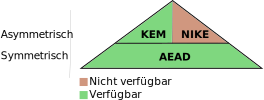
\includegraphics[height=.6\textheight]{graphics/Primitivenpyramide.pdf}
      
    Die meisten Protokolle inklusive WireGuard nutzen NIKEs    
\end{frame}

%%%%%%%%%%%%%%%%%%%%%%%%%%%%%%%%%%%%%%%%%%%%%%%
% Rosenpass Demo

\begin{frame}{Rosenpass Demo!}
  \includegraphics[height=.9\textheight]{assets/2023-03-20-rg-tutorial-screenshot.png}
\end{frame}

%%%%%%%%%%%%%%%%%%%%%%%%%%%%%%%%%%%%%%%%%%%%%%%%
%% Wie funktioniert Rosenpass

\begin{frame}{Verschlüsselung im Angesicht von Quantencomputern}
    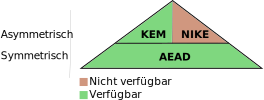
\includegraphics[height=.6\textheight]{graphics/Primitivenpyramide.pdf}
      
    Die meisten Protokolle inklusive WireGuard nutzen NIKEs    
\end{frame}

\begin{frame}{Schlüsseltauschmethoden: Mit NIKEs\footnote{\say{Non-interactive key exchange} -- Nichtinteraktiver Schlüsseltausch}}
\usetikzlibrary{shapes,decorations,decorations.pathreplacing,arrows,calc,arrows.meta,fit,chains,positioning,shadows}
\begin{tikzpicture}[
rosenpass-diagram,
  % define multiple syles for consistency
  boxed-node/.style = {draw, rectangle, fill=white, text width = 5em, align = center, minimum height = 1.75em, rounded corners},
  swimming-lane/.style = {very thick},
  message-flow/.style = {-{Stealth[length = 0.5em]}, shorten >= 0.25em, shorten <= 0.25em},
]

  % iterate over i, multiply with 1cm, creating a vertical, down moving row of coordinates
  \foreach \i [evaluate=\i as \angle using { \i * 1cm}] in {0,...,5}
    \coordinate (n-\i) at (0,-\i);

  % set two initial nodes, positioned relative to the coordinates
	 \draw[initiator](-1,0) node(initiator){Initiator} coordinate(ini) ++(0,.1)to
		coordinate[pos=.2](spki-y)
		coordinate[pos=.6](spkr-y)
		coordinate[pos=.76](ack-y)+(0,-5) coordinate(result-y);
	  \draw[responder] (1,0) node(responder){Response} coordinate (res)++(0,.1)to +(0,-5);
%  \node[boxed-node] (ini) at (n-0) {Initiator};
%  \node[boxed-node,right = of ini] (res) {Response};

  % place a text on the intersection of the ini node and the n-1 coordinate
  \node[anchor = east] (sski) at (n-1 -| ini) {(sski, spki) $\leftarrow$ keygen()};

  % place a text on the intersection of the res node and the n-2 coordinate
  \node[anchor = west] (sskr) at (n-2 -| res) {(sskr, spkr) $\leftarrow$ keygen()};

  % place text on below ini and res node on the height of the n-3 coordinate
  \node[anchor = east] (dhi) at (n-4 -| ini) {key $\leftarrow$ dh(sski, spkr)};
  \node[anchor = west] (dhr) at (n-4 -| res) {key $\leftarrow$ dh(sskr, spki)};

  % TODO: Horizontale (gestrichelte) linie um zu zeigen wo das setup endet?

  % define the vertical swimming lanes
%  \begin{scope}[style = swimming-lane]
%     \draw (ini) -- (n-5 -| ini);
%     \draw (res) -- (n-5 -| res);
%  \end{scope}

  % define the message flows
  \begin{scope}[style = message-flow]
     \draw [request](sski) -- node[above]{spki} (sski -| res);
     \draw [response](n-2 -| ini) -- node[above]{spkr} (n-2 -| res);
  \end{scope}
\end{tikzpicture}

Static-static Schlüsseltausch mit NIKEs.

\end{frame}

\begin{frame}{Schlüsseltauschmethoden: Mit KEMs\footnote{\say{Key-Encapsulation Method} -- Schlüsselverpackungsmethode} wird es komplizierter}
\begin{tikzpicture}[
  % define multiple syles for consistency
  boxed-node/.style = {draw, rectangle, fill=white, text width = 5em, align = center, minimum height = 1.75em, rounded corners},
  swimming-lane/.style = {very thick},
  message-flow/.style = {-{Stealth[length = 0.5em]}, shorten >= 0.25em, shorten <= 0.25em},
]

  % iterate over i, multiply with 1cm, creating a vertical, down moving row of coordinates
  \foreach \i [evaluate=\i as \angle using { \i * 1cm}] in {0,...,6}
    \coordinate (n-\i) at (0,-\i);

  % set two initial nodes, positioned relative to the coordinates
  \node[boxed-node] (ini) at (n-0) {Initiator};
  \node[boxed-node,right = of ini] (res) {Response};

  % place a text on the intersection of the ini node and the n-1 coordinate
  \node[anchor = east] (sski) at (n-1 -| ini) {(sski, spki) $\leftarrow$ keygen()};

  % place a text on the intersection of the res node and the n-2 coordinate
  \node[anchor = west] (sskr) at (n-2 -| res) {(sskr, spkr) $\leftarrow$ keygen()};

  % place a text on the intersection of the res node and the n-2 coordinate
  \node[anchor = east] (sctr) at (n-4 -| ini) {(key1, sctr) $\leftarrow$ encaps(spkr)};
  \node[anchor = west] (decapsr) at (n-4 -| res) {key1 $\leftarrow$ decaps(sctr)};

  \node[anchor = west] (scti) at (n-5 -| res) {(key2, scti) $\leftarrow$ encaps(spki)};
  \node[anchor = east] (decapsi) at (n-5 -| ini) {key2 $\leftarrow$ decaps(scti)};

  % define the vertical swimming lanes
  \begin{scope}[style = swimming-lane]
     \draw (ini) -- (n-6 -| ini);
     \draw (res) -- (n-6 -| res);
  \end{scope}

  % define the message flows
  \begin{scope}[style = message-flow]
     \draw (sski) -> node[above]{spki} (sski -| res);
     \draw (n-2 -| res) -> node[above]{spkr} (n-2 -| ini);

     \draw (sctr) -> node[above]{sctr} (sctr -| res);
     \draw (n-5 -| res) -> node[above]{scti} (n-5 -| ini);
  \end{scope}
\end{tikzpicture}

Static-static Schlüsseltausch mit KEMs.

\end{frame}

\begin{frame}{Einfachst-möglicher Schlüsseltausch mit KEMs}
\begin{tikzpicture}[
  % define multiple syles for consistency
  boxed-node/.style = {draw, rectangle, fill=white, text width = 5em, align = center, minimum height = 1.75em, rounded corners},
  swimming-lane/.style = {very thick},
  message-flow/.style = {-{Stealth[length = 0.5em]}, shorten >= 0.25em, shorten <= 0.25em},
]

  % iterate over i, multiply with 1cm, creating a vertical, down moving row of coordinates
  \foreach \i [evaluate=\i as \angle using { \i * 1cm}] in {0,...,6}
    \coordinate (n-\i) at (0,-\i);

  % set two initial nodes, positioned relative to the coordinates
  \node[boxed-node] (ini) at (n-0) {Initiator};
  \node[boxed-node,right = of ini] (res) {Response};

  % place a text on the intersection of the res node and the n-2 coordinate
  \node[anchor = west] (sskr) at (n-1 -| res) {(sskr, spkr) $\leftarrow$ keygen()};

  % place a text on the intersection of the res node and the n-2 coordinate
  \node[anchor = east] (sctr) at (n-3 -| ini) {(key, sctr) $\leftarrow$ encaps(spkr)};
  \node[anchor = west] (decapsr) at (n-3 -| res) {key $\leftarrow$ decaps(sctr)};

  % define the vertical swimming lanes
  \begin{scope}[style = swimming-lane]
     \draw (ini) -- (n-6 -| ini);
     \draw (res) -- (n-6 -| res);
  \end{scope}

  % define the message flows
  \begin{scope}[style = message-flow]
     \draw (n-1 -| res) -> node[above]{spkr} (n-1 -| ini);
     \draw (sctr) -> node[above]{sctr} (sctr -| res);
  \end{scope}
\end{tikzpicture}
\end{frame}

\begin{frame}{Post-quantum WireGuard: Three encapsulations}
\begin{columns}[onlytextwidth]

\begin{column}{.30\textwidth}
\begin{tikzpicture}[rosenpass-diagram]
	 \draw[initiator] (-1,0) node(initiator){Initiator} ++(0,.1)to
		coordinate[pos=.2](spki-y)
		coordinate[pos=.6](Hspki-y)
		coordinate[pos=.76] (scti-y)
		coordinate[pos=.92](ack-y)+(0,-5);
	 \draw[responder] (1,0) node (responder){Responder} ++(0,.1)to+(0,-5)coordinate(result-y);;

	 \draw[request](spki-y-|initiator) -- node[above]{spki} (spki-y-|responder);
	 \draw[request](Hspki-y-|initiator) -- node[above] {H(spki)} (Hspki-y-|responder);

	  \draw[response,response](scti-y-|initiator) -- node[above]{scti} (scti-y-|responder);

	 \draw[request](ack-y-|initiator) -- node[above] {(ack)} (ack-y-|responder);
	\path[result] node at (result-y-|0,0){Initiator Auth};
\end{tikzpicture}
\end{column}

\begin{column}{.30\textwidth}
\begin{tikzpicture}[rosenpass-diagram]
	 \draw[initiator](-1,0) node(initiator){Initiator} ++(0,.1)to
		coordinate[pos=.2](spkr-y)
		coordinate[pos=.6](sctr-y)
		coordinate[pos=.76](ack-y)+(0,-5) coordinate(result-y);
	  \draw[responder] (1,0) node(responder){Responder} ++(0,.1)to +(0,-5);
		\draw[response](spkr-y-|initiator) -- node[above]{spkr} (spkr-y-|responder);
		\draw[request](sctr-y-|initiator) -- node[above] {sctr} (sctr-y-|responder);
		\draw[response](ack-y-|initiator) -- node[above] {(ack)} (ack-y-|responder);
	\path[result] node at (result-y-|0,0){Responder Auth};
\end{tikzpicture}
\end{column}


\begin{column}{.30\textwidth}
\begin{tikzpicture}[rosenpass-diagram]
	 \draw[initiator] (-1,0) node(initiator){Initiator}  ++(0,.1)to
		coordinate[pos=.6](epki-y)
		coordinate[pos=.76] (ecti-y)
		coordinate[pos=.92](ack-y)+(0,-5);
	 \draw[responder] (1,0) node(responder){Responder} ++(0,.1)to +(0,-5)coordinate(result-y);;

	 \draw[request](epki-y-|initiator) -- node[above]{epki} (epki-y-|responder);
	 \draw[response](ecti-y-|initiator) -- node[above]{ecti} (ecti-y-|responder);
	 \draw[request](ack-y-|initiator) -- node[above] {(ack)} (ack-y-|responder);
	\path[result] node at (result-y-|0,0){Forward secrecy};
\end{tikzpicture}
\end{column}

\end{columns}
\end{frame}

\begin{frame}{Combining the three encapsulations in one protocol}

\begin{tikzpicture}[rosenpass-diagram]
	\draw[initiator] (-3,0) node(initiator){Initiator}  ++(0,.1)to coordinate[pos=.2](spki-y)
	coordinate[pos=.35](spkr-y)
	coordinate[pos=.6](epki-y)
	coordinate[pos=.75](scti-y)
	coordinate[pos=.9](ack-y)+(0,-5);
	\draw[responder] (3,0) node(responder){Responder} ++(0,.1)to+(0,-5);

	 \draw[request](spki-y-|initiator) -- node[above] {spki} (spki-y-|responder);
	 \draw[response](spkr-y-|initiator) -- node[above] {spkr} (spkr-y-|responder);
	 \draw[request](epki-y-|initiator) -- node[above] {epki, sctr, H(spki)} (epki-y-|responder);
	 \draw[response](scti-y-|initiator) -- node[above] {scti,ecti} (scti-y-|responder);
	  \draw[request](ack-y-|initiator) -- node[above] {(ack)} (ack-y-|responder);

\end{tikzpicture}

  Note that the initiator is not authenticated until they send \enquote{(ack)}.

\end{frame}

\begin{frame}{The Rosenpass protocol}
  \includegraphics[height=.9\textheight]{graphics/rosenpass-wp-key-exchange-protocol-rgb.pdf}
\end{frame}

\begin{frame}{Sicherheitsanalyse}
  \begin{itemize}
    \item Softwarebeweise sind quasi tests für jeden möglichen Input
    \item Wir nutzen ProVerif als tool um Protokoll-Bugs auszuschließen
    \item Wir arbeiten an besseren Beweisen (mit Cryptoverif)
    \item Beweise sind teil der Software; laufen in der CI
    \item Wir haben die Laufzeit optimiert; symbolische analyse läuft in fünf Minuten
  \end{itemize}
\end{frame}

\begin{frame}{Proverif in technicolor}
  \includegraphics[height=.9\textheight]{assets/2023-03-20-symbolic-analysis-screenshot.png}
\end{frame}

\begin{frame}{Rosenpass/WireGuard integration}
  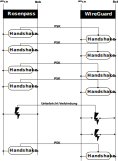
\includegraphics[height=.9\textheight]{graphics/rpwg.pdf}
\end{frame}

\begin{frame}{Chiffren}
  \begin{itemize}
    \item Authentifikation \& Geheimheit: \textbf{Classic McEliece} (erfunden 1979, Codebasiert)
    \item Forward Secrecy: \textbf{Kyber} (NIST-Standardisiert, Gitter)
    \item Wir planen die Möglichkeit die Chiffren zu wechseln einzubauen
  \end{itemize}
\end{frame}

\begin{frame}{Ausblick}
  \begin{itemize}
    \item Sicherheitsbeweis im probabilistischen Model mit Cryptoverif
    \item Möglichkeit Chiffren zu wechseln
    \item Möglichkeit Post-Quantum Chiffren einzubauen (Hybride Sicherheit)
    \item Möglichkeit mehrere Chiffren gleichzeitig zu verwenden
    \item Rosenpass in Kubernetes
    \item Isolation, Micro-VMs, Docker
    \item Formell verifizierte Implementierung
    \item Mehr WissKomm zu Kryptografie. Kryptografie braucht verständliche Erklärungen!
  \end{itemize}
  \begin{itemize}
    \item Wir suchen High-Assurance Kryptografieprojekte um mit uns zusammenzuarbeiten. Rosenpass ist klein und kann als Demonstrator dienen.
  \end{itemize}
\end{frame}

\begin{frame}{Zum nachbauen… aus dem Whitepaper:}
  \includegraphics[height=.9\textheight]{graphics/rosenpass-wp-message-handling-code.pdf}
\end{frame}

% TODO: Posterfolie? KEMs statt Diffie-Hellmann; 

\maketitle

%%%%%%%%%%%%%%%%%%%%%%%%%%%%%%%%%%%%%%%%%%%%%%%

\begin{frame}{CVE-2021-46873 – DOS against WireGuard through NTP}
\begin{itemize}
  \item The replay protection in classic WireGuard assumes a monotonic counter
  \item But the system time is attacker controlled because NTP is insecure
  \item This generates a kill packet that abuses replay protection and renders the initiator's key-pair useless
  \item Attack is possible in the real world!
  \item Similar attack in post-quantum WireGuard is worse since InitHello is unauthenticated
  \item Solution: Biscuits
\end{itemize}
\end{frame}

\begin{frame}{New Hashing/Domain separation scheme}
  \includegraphics[height=.9\textheight]{graphics/rosenpass-wp-hashing-tree.pdf}
\end{frame}

\end{document}
